%%
% Please see https://bitbucket.org/rivanvx/beamer/wiki/Home for obtaining beamer.
%%
\documentclass[aspectratio=43, 10pt]{beamer}

\setbeamercolor{structure}{fg=gray}
\setbeamercolor{palette sidebar secondary}{fg=black,bg=white}
\setbeamertemplate{section in toc}[sections numbered]
\addtobeamertemplate{footnote}{}{\vspace{2ex}}

\usetheme{Goettingen}
\usecolortheme{dove}

\setbeamerfont{frametitle}{series=\bfseries,parent=structure}

\usepackage{listings}
\usepackage{lmodern}
\usepackage[utf8]{inputenc}
\usepackage{xcolor}
\usepackage{multicol}
\usepackage{graphicx}
\usepackage{parskip}
%\usepackage{fontspec}
%\usepackage{helvet}
\usepackage{../../tikzit}

\definecolor{uqcs}{HTML}{6297CD}

%\setsansfont[BoldFont={* Bold}]{SF Pro Display}
%\setmonofont[Scale=0.95]{SF Mono}

\input{../../styles.tikzstyles}

\lstset{basicstyle=\color{uqcs}\ttfamily, basewidth=0.5em}
\lstMakeShortInline[columns=fixed]|

\title{The \textbf{\TeX} Talk}
\subtitle{Programming Perfect Documents}
\author{Matthew Low\\\color{uqcs}UQCS\\\vspace{1.5em}
\includegraphics[width=0.2\textwidth]{figures/uqcs}}
\date{April 7, 2020}

\begin{document}

\begin{frame}
\centering
\vspace{2em}
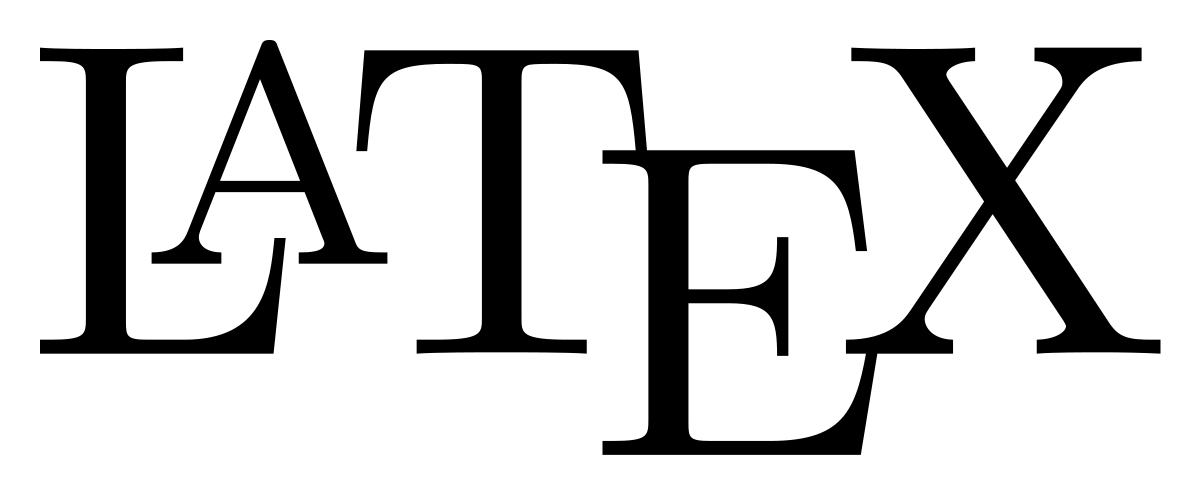
\includegraphics[width=0.3\textwidth]{figures/latexlogo}
\maketitle	
\end{frame}

\begin{frame}{Meme}
\centering

\includegraphics[height=0.7\textheight]{figures/meme}
\end{frame}

\begin{frame}{Motivation}
	Writing Microsoft Word documents can sometimes be a painful experience. This is mostly caused by the clunky interface and Word's focus on layout rather than content; you need to do a lot of layout work on your own to get an appealing document.
\end{frame}

\begin{frame}{Motivation}
	\LaTeX \ aims to shift the focus to \textbf{content}. \LaTeX \ will handle all of the heavy-lifting (what page should this paragraph should be on? where should this image go?) and let you focus on the content.
\end{frame}

\begin{frame}{Outline}
\begin{multicols}{2}
	\tableofcontents
	\end{multicols}	
\end{frame}

\section{How \LaTeX \ works}

\begin{frame}{What is \LaTeX, and what is \TeX?}

\LaTeX \ is a document \textbf{typesetting system}.

\TeX \ is its \textbf{programming language}\footnote{Actually, it's quite complicated and confusing (\TeX is also a typesetting system). But this is a good place to start.}.

\LaTeX \ is pronounced LAY-tek or LAH-tek, \textit{not} LAY-teks.
\end{frame}

\begin{frame}[fragile]{How does \LaTeX \ work?}
In the most simple terms possible...

\begin{tikzpicture}
	\begin{pgfonlayer}{nodelayer}
		\node [style=rectangle] (0) at (0, 0) {\TeX \ code (\texttt{.tex})};
		\node [style=rectangle] (1) at (3.7, 0) {\LaTeX \ compiler};
		\node [style=rectangle] (2) at (7, 0) {PDF output};
	\end{pgfonlayer}
	\begin{pgfonlayer}{edgelayer}
		\draw [style=arrow] (0) to (1);
		\draw [style=arrow] (1) to (2);
	\end{pgfonlayer}
\end{tikzpicture}
\end{frame}

\begin{frame}{How does \LaTeX \ work?}
	\begin{itemize}
		\item<1-> \textbf{Editing \TeX \ code?} Any text editor will do, though VSCode, Vim, emacs with plugins are popular options. There are also IDEs such as TeXstudio/TeXmaker etc.
		\item<2-> \textbf{Running the \LaTeX \ compiler?} pdfLaTeX, XeLaTeX, LuaLaTeX (we will only cover pdfLaTeX today).
		\item<3-> How do I get the compilers, packages, and other stuff? Download a \textbf{\LaTeX \ distribution}. Popular options are MiKTeX for Windows, TeX Live for Linux/UNIX, MacTeX for macOS. Alternatively, you can use a website like Overleaf and everything is handled in the browser! \textbf{This is recommended for beginners. Free premium accounts for UQ students!}
	\end{itemize}
\end{frame}

\begin{frame}{Before we start diving in...}
	\Large A TeX file is a program. 
	
	This can be good or bad.
	
	You need to write \textbf{correct} code, or else LaTeX can't magically compile it for you.
\end{frame}

\begin{frame}{Before we start diving in...}
	You \textit{will} get syntax errors. Writing documents and getting syntax errors may be a weird experience for you, but learning how to identify and fix those errors over time will help you understand and appreciate greatly the LaTeX system.
\end{frame}

\section{Basic document}

\begin{frame}[fragile]{Something simple...}
This is about as simple as it gets for TeX.
\begin{lstlisting}
\documentclass{article}
\begin{document}
Hello!
\end{document}
\end{lstlisting}
\end{frame}

\begin{frame}{Something simple...}
Typing this and compiling will give you a page that looks like this...


\centering

\includegraphics[height=0.7\textheight]{figures/1}
\end{frame}

\begin{frame}[fragile]{What are these bits of code?}
	\begin{itemize}
		\item<1-> |\documentclass{article}| says that the \textbf{document class} should be of type `article'. There are other classes, such as `book', `report' etc. This will become important later when we talk about sections.
		\item<2-> |\begin{document}| starts a new ``document''. Every thing past here goes on the page, or affects the page.
		\item<3-> |\end{document}| should be the last line of every TeX document you write.
	\end{itemize}
\end{frame}

\begin{frame}[fragile]{Environments}
|\begin| and |\end| are delimiters for an \textbf{environment}. In \LaTeX, almost everything is an environment. You will see this soon.
\end{frame}

\begin{frame}[fragile]{Document structure}
Note the code below.
\begin{lstlisting}
\documentclass{article}
\begin{document}
Hello!
\end{document}
\end{lstlisting}
Everything above the |\begin{document}| is part of what is called the \textbf{preamble}. This is where you setup the document.

\end{frame}

\begin{frame}[fragile]{Starting off a document}
	Maybe you want a bit more than ``Hello!'' in a document. Maybe you want to start with a title? Author? Date? Simple as. Put this in the \textbf{preamble}:

\begin{lstlisting}
\title{My Document!}
\author{Me}
\date{\today}
\end{lstlisting}

|\today| is a command which returns the current date.
\end{frame}

\begin{frame}[fragile]{Starting off a document}
Our full code now looks like this:
\begin{lstlisting}
\documentclass{article}
\title{My Document!}
\author{Me}
\date{\today}
\begin{document}
Hello!
\end{document}
\end{lstlisting}
Cool! Let's run it...
\end{frame}

\begin{frame}[fragile]{Starting off a document}
\centering

\includegraphics[height=0.7\textheight]{figures/1}

...wait, where's my title?
\end{frame}

\begin{frame}[fragile]{Starting off a document}
No worries, just have to actually print the title. Remember, the title, author and date are specified in the preamble, so it won't show up in the document until we say to print it. In this case, we need to add

|\maketitle|

after |\begin{document}| to get it to actually show up.
\end{frame}

\begin{frame}[fragile]{Starting off a document}
\centering

\includegraphics[height=0.7\textheight]{figures/2}

Better!
\end{frame}

\begin{frame}[fragile]{Structure}
	The next thing your document needs is some structure. To do this, we will make use of a command called
	
	|\section|.
	
	There is also
	
	|\subsection|, |\subsubsection|, ..., |\chapter|, |\part| etc.
	
	The availability of these depends on your document class. For example, articles don't have chapters; books do.
\end{frame}

\begin{frame}[fragile]{Table of contents}
	To do a table of contents, type the code
	
	|\tableofcontents|
	
	in your documents. It will automatically be generated from the sections that you specified with |\section|, |\subsection| etc.
\end{frame}

\begin{frame}{We're done!}
	Now, we technically have everything we need to start writing our 500-page novel. But, of course, there may be a few fancier things than paragraphs that we may want to add.
	
	Images? Tables? Lists? Code? Math?
	\end{frame}

\section{Environments}

\begin{frame}[fragile]{Images and figures}
	To put an image on the page, you need to have the |graphicx| package imported. A package is essentially an ``add-on'' that adds more features, environments and options in your document. We'll see more of these as we go on.
	
	To import |graphicx|, type in the preamble:
	
	\begin{lstlisting}
\usepackage{graphicx}
	\end{lstlisting}
	We can create an image by simply putting
	
	\begin{lstlisting}
\includegraphics{path_to_image}
	\end{lstlisting}
	
	in the document. But this might make a massive image, or a tiny one! And it's not centered!
\end{frame}

\begin{frame}[fragile]{Images and figures}
To fix this, we can create a center environment:
	
	\begin{lstlisting}
\begin{center}
    \includegraphics{path_to_image}
\end{center}
    \end{lstlisting}
     
\pause and also specify a width with an \textbf{option} to |\includegraphics|:
     
    \begin{lstlisting}
\begin{center}
    \includegraphics[width=0.6\textwidth]
                    {path_to_image}
\end{center}
    \end{lstlisting}

|\textwidth| is a ``length'' for the width of the current area of text. There are many other lengths specified in TeX.

\end{frame}

\begin{frame}[fragile]{Figures}
	Another method of putting an image on the screen is using a figure environment. This can be done by wrapping the |\includegraphics| in it like so:
	\begin{lstlisting}
\begin{figure}
    \centering
    \includegraphics[width=0.6\textwidth]
                    {path_to_image}
    \caption{This is a wonderful image!}
\end{figure}
\end{lstlisting}

\pause

The |\centering| is equivalent to wrapping in a |\begin{center}| and |\end{center}|, but it is a toggle. Since it is called inside an environment, it stops centering after the environment is finished. If you typed |\centering| in the main body of the document, it would center everything (including text) until the end.

\pause

|\caption{}| does exactly what it says.
\end{frame}

\begin{frame}[fragile]{Float}
	You may notice that figures don't really go where you want them to go. This is all part of \LaTeX's smarts.
	
	To fix this, simply import the package	
	|\usepackage{float}|
	
	and put a |[H]| after |\begin{figure}|, like so:
	\begin{lstlisting}
\begin{figure}[H]
    \centering
    \includegraphics[width=0.6\textwidth]
                    {path_to_image}
\end{figure}
\end{lstlisting}
	This will force the image to go exactly where you specified.

\end{frame}

\begin{frame}[fragile]{Tables}
	Tables are quite simple. To make a 3 column table where all columns are centre-aligned:
	\begin{lstlisting}
\begin{tabular}{ccc}
    a & b & c \\
    d & e & f	
\end{tabular}
	\end{lstlisting}
	
	|&| is the ``alignment'' character in TeX, and |\\| are the ``linebreak'' characters. You'll see these a lot in maths.
	
	|l| for left aligned, |c| for centered, |r| for right-aligned. If you want to center the whole table, use a figure or |\begin{center}|.
\end{frame}

\begin{frame}[fragile]{Ordered and unordered lists}
	Ordered lists are called \textbf{enumerates}. Unordered lists are called \textbf{itemizes}. To do them, simply:
	
	\begin{lstlisting}
\begin{enumerate}
    \item Hello
    \item Hi
\end{enumerate}
	\end{lstlisting}
	
	or
	
	\begin{lstlisting}
\begin{itemize}
    \item Hello
    \item Hi
\end{itemize}
	\end{lstlisting}
\end{frame}

\section{Text formatting}

\begin{frame}[fragile]{Font sizes}
	Font sizes are based off of the \textbf{base font size}. This is set in the document class by default to 10pt. If you want 11pt, or 12pt, provide the command 11pt or 12pt as an argument to the document class.
	
	
\end{frame}

\begin{frame}[fragile]{Bold, italic and underline}
	To apply formatting to text, it is often useful to wrap it in some command such as |\textbf|. For example:
	\begin{itemize}
		\item To \textbf{bold} text, |\textbf{the text}| or |\bfseries| to switch.
		\item To \textit{italicise} text, |\textit{the text}| or |\itshape| to switch.
		\item To \underline{underline} text, |\underline{the text}| (it doesn't have a switch, but you can define one.)
	\end{itemize}
\end{frame}

\begin{frame}[fragile]{Left align, right align and centre}
	You can align text both as a switch and as an environment. 
	\begin{itemize}
		\item To \textbf{left-align}, use the |\begin{flushleft}|, or use the |\raggedright| switch.
		\item To \textbf{right-align}, use the |\begin{flushright}|, or use the |\raggedleft| switch.
		\item To \textbf{centre-align}, use the |\begin{center}|, or use the  |\centering| switch.
		\item To \textbf{justify} (default), use the |\justify| switch.	
	\end{itemize}
\end{frame}

\section{Packages}

\begin{frame}{Packages}
	\Large Let's look at more packages.
\end{frame}

\begin{frame}[fragile]{Essential packages}
	We've already covered |graphicx| and |float|. Now, I'll cover 
	\begin{itemize}
		\item |listings| for writing code and syntax highlighting;
		\item |amsmath, amsthm, amssymb| for writing mathematics (theorems and proofs);
		\item |geometry| for adjusting page dimensions;
		\item |biblatex| for bibliographies
	\end{itemize}
\end{frame}

\section{Code listings}

\begin{frame}[fragile]{Code listings}
	To write code, use the |listings| package, and write in your document:
	\color{uqcs}\begin{verbatim}
\begin{lstlisting}
def hello_world():
    print("Hello world!")
\end{lstlisting}
	\end{verbatim}\color{black}
	This will print the code in its own nice little environment. 
	\pause
	You might want to syntax highlight too: you can do this by providing the option |[language=python]| in this case, with an output like:
	\begin{lstlisting}[language=Python]
def hello_world():
    print("Hello world!")
	\end{lstlisting}
	You can see how it \textit{slightly} bolds |def| and |print|, and puts a space character in. Syntax highlighting varies by language, and you can do a whole bunch more than this. Just google.
\end{frame}

\begin{frame}[fragile]{External code}
	Do you want code from another file?Just use |\lstinputlisting|.
	
	\begin{lstlisting}
\lstinputlisting{name_of_code.py}
	\end{lstlisting}
	
	This will place the code from the file |name_of_code.py| in that position.
\end{frame}

\section{Mathematics}

\begin{frame}[fragile]{Writing math}
	So, you want to write some mathematics. LaTeX is \textbf{the} tool for typesetting mathematics. Its syntax is super simple, and very easy to get the hang of. I'll go through some basics here. \pause
	
	For this section onwards, we assume we have imported the |ams| packages |amsmath| (basics), |amssymb| (more symbols) and |amsthm| (theorem environments). \pause
	
	Firstly, there are two types of math environments: \textbf{inline} and \textbf{display}. Inline is done using |$$| and |\(\)|, whereas display math is typically done using |$$$$| and |\[\]|. Most people use |$$| and |\[\]| for technical reasons (spacing).
	
	Inline math goes inline, like this $\sin^2 \theta + \cos^2 \theta = 1$. Display math goes ``out-of-line'', like this \[\sin^2 \theta + \cos^2 \theta = 1.\]
\end{frame}

\begin{frame}[fragile]{Writing math}
	Plus and minus are just typed on the keyboard. Multiplication ($\times$) is written using |\times|. Fractions ($\frac{a}{b}$) are written using |\frac{a}{b}|. \pause
	
	Common operators and symbols are written using |\nameofsymbol|. If you are applying some operator or function to some variables, you might need curly brackets. For example, |\sqrt{a}| gives $\sqrt{a}$. \pause 
	
	Trigonometric functions are written as expected (|\sin|, |\cos|, |\tan| give $\sin, \cos, \tan$). Exponentials and logarithms are also self-explanatory. \pause
	
	To write lowercase, write |\delta| ($\delta$) for example (note the lowercase `a'). For uppercase, |\Delta| ($\Delta$). 
\end{frame}

\begin{frame}[fragile]{Writing more advanced math}
	Powers and subscripts are written using |_{}| and |^{}|. For example, |x^2| gives $x^2$ and |x_1| gives $x_1$. \pause

	For operators with limits (limits, integrals), you denote the lower limit by |_{}| and upper limit by |^{}|, for example |\int_{-\infty}^{\infty}| = $\int_{-\infty}^\infty$. \pause
	
	Parentheses with fractions do not ``stretch'' by default. If you want them to, wrap the parentheses (or whatever other brackets) in |\left| and |\right|. For example, |\[\left(\frac{1}{2}\right)\]| will give 
	\[
		\left(\frac{1}{2}\right)
	\] 
	whereas |\[(\frac{1}{2})\]| will give
	\[
		(\frac{1}{2}).
	\]
\end{frame}

\begin{frame}[fragile]{Writing more advanced math}
	Matrices are done using the \textbf{matrix} environment, \textbf{inside a math environment}. You can wrap matrices in a |\left(| and |\right)| to obtain ``pmatrices'', or you can use the package |amsmath| to use the \textbf{pmatrix} environment directly. Matrices are done the same way as tables, but without column specification:
	\begin{lstlisting}
\[
  \begin{matrix}
    a & b & c \\
    d & e & f \\
    g & h & i
  \end{matrix}
\]
	\end{lstlisting}
	\[
  \left(\begin{matrix}
    a & b & c \\
    d & e & f \\
    g & h & i
  \end{matrix}\right)
\]
\end{frame}

\begin{frame}[fragile]{Mathematical alphabets}
	You may find yourself needing to use fancier mathematical alphabets in certain situations. Note that these alphabets are different to |\textbf| etc. that we defined above as these can only be used in math mode. There are plenty more than just these.
	\pause
	\begin{itemize}
		\item |\mathrm| is roman (upright) $\mathrm{ABC}$
		\item |\mathit| is italic (the default, keep this in mind when writing operators as upright is convention) $\mathit{ABC}$
		\item |\mathsf| is sans-serif (this document is sans so it looks ``normal'') $\mathsf{ABC}$
		\item |\mathbf| is bold $\mathbf{ABC}$	
		\item |\mathbb| is blackboard bold $\mathbb{ABC}$
		\item |\mathcal| is calligraphic $\mathcal{ABC}$
		\item |\mathfrak| is Fraktur $\mathfrak{ABC}$
	\end{itemize}
\end{frame}

\begin{frame}[fragile]{Now, you can write this!}
	\[\int_{-\infty}^{\infty} \frac{1}{\sqrt{2\pi\sigma^2}} e^{\frac{-(x-\mu)^2}{2\sigma^2}} \mathrm{d}x = 1\]
	can be written using the LaTeX code
	\begin{lstlisting}
\[
  \int_{-\infty}^{\infty} \frac{1}{\sqrt{2\pi\sigma^2}}
  e^{\frac{-(x-\mu)^2}{2\sigma^2}} \mathrm{d}x = 1
\]
	\end{lstlisting}
	Want to practice writing math? Go to TeXnique! It's a fun web game which gives you a bunch of equations to type within a time limit. \href{https://texnique.xyz/}{\color{uqcs}\texttt{https://texnique.xyz/}}
\end{frame}

\begin{frame}[fragile]{Aligned math}
	If you have multiple lines of math you want aligned, you can use an \textbf{align*} or \textbf{align} environment. The * indicates no numbered labels.
	
	For example, typing
	\begin{lstlisting}
\begin{align*}
	\sin^2 \theta + \cos^2\theta &= 1 \\
	\tan^2 \theta + 1 &= \sec^2 \theta \\
	1 + \cot^2 \theta &= \csc^2 \theta	
\end{align*}
	\end{lstlisting}
	will give you
\begin{align*}
	\sin^2 \theta + \cos^2\theta &= 1 \\
	\tan^2 \theta + 1 &= \sec^2 \theta \\
	1 + \cot^2 \theta &= \csc^2 \theta	
\end{align*}
Note the alignment character |&|.
\end{frame}

\begin{frame}[fragile]{Theorem environments}
	To create a theorem environment, we first have to define one. Put this in the preamble:
	\begin{lstlisting}
\newtheorem{theorem}{Theorem}
	\end{lstlisting}
	You can then create a theorem anywhere in the text by typing
	\begin{lstlisting}
\begin{theorem}
	UQCS is a wonderful organisation.	
\end{theorem}
	\end{lstlisting}
	\begin{theorem}
	UQCS is a wonderful organisation.	
\end{theorem}
\end{frame}

\begin{frame}[fragile]{Proof environment}
	Proofs are already defined for us, just use the proof environment. It even puts a cute square box at the end!
	\begin{lstlisting}
\begin{theorem}
  UQCS is a wonderful organisation.	
\end{theorem}
\begin{proof}
  Left as an exercise for the reader.	
\end{proof}
	\end{lstlisting}
	
\begin{theorem}
  UQCS is a wonderful organisation.	
\end{theorem}
\begin{proof}
  Left as an exercise for the reader.	
\end{proof}
	
\end{frame}

\begin{frame}{Mathematics in LaTeX: a summary}
	\Large There is a \textbf{lot} of math stuff in LaTeX. Just keep practicing and you'll be fluent in no time!
\end{frame}

\section{Document formatting and referencing}

\begin{frame}[fragile]{Footnotes}
	To put a footnote in your document, simply type |\footnote{This is a footnote!}|\footnote{This is a footnote!}
\end{frame}

\begin{frame}[fragile]{Bibliographies}
	To create a bibliography, use the package |biblatex|, create a |.bib| file (BibLaTeX file) and link it in the preamble using the syntax
	\begin{lstlisting}
\addbibresource{name_of_bib_file.bib}		
	\end{lstlisting}
	This allows you to reference any entries in the |.bib| file using |\cite{}| in the body of the |.tex| file, where the label of the reference in the |.bib| file is inserted in the curly brackets. To print the bibliography somewhere in the document, simply type
	\begin{lstlisting}
\printbibliography
	\end{lstlisting}
\end{frame}

\begin{frame}[fragile]{Sample .bib file}
	Here's an example of a |.bib| file, courtesy of Overleaf:
	\begin{lstlisting}[basicstyle=\ttfamily\color{uqcs}\scriptsize]
@article{einstein,
    author =       "Albert Einstein",
    title =        "{Zur Elektrodynamik bewegter K{\"o}rper}. ({German})
    [{On} the electrodynamics of moving bodies]",
    journal =      "Annalen der Physik",
    volume =       "322",
    number =       "10",
    pages =        "891--921",
    year =         "1905",
    DOI =          "http://dx.doi.org/10.1002/andp.19053221004",
    keywords =     "physics"
}

@online{knuthwebsite,
    author    = "Donald Knuth",
    title     = "Knuth: Computers and Typesetting",
    url       = "http://www-cs-faculty.stanford.edu/~uno/abcde.html",
    keywords  = "latex,knuth"
}
	\end{lstlisting}
	Many bibliography managers can export to BibLaTeX.
\end{frame}

\begin{frame}[fragile]{Include and input}
	This is really important and really cool. You can put other |.tex| files in your current |.tex| file by using the commands
	
	\begin{lstlisting}
\include{the_sub_tex_file.tex}
	\end{lstlisting}
	or
	\begin{lstlisting}
\input{the_sub_tex_file.tex}		
	\end{lstlisting}
	
	This allows you to modularise all of your documents to subfiles, and even strip out a common preamble to apply to all of your documents!\footnote{The difference between input and include is that input purely inserts the sub-file's TeX in that position in the document, whereas include does some fancy stuff with .aux files to speed up compilation, and also adds page breaks.}
\end{frame}

\begin{frame}[fragile]{Margins and page size}
	Want to adjust the margins of your page? More importantly, would you like to print your documents at A4 size (since US Letter is the default in LaTeX, you will want to do this for 1-to-1 printing without scaling)?
	
	Simply import the |geometry| package, and use the |\geometry| command in your preamble to specify parameters. For example:
	
	\begin{lstlisting}
\geometry{left=2cm, right=2cm, 
          bottom=3cm, top=3cm, a4paper}
	\end{lstlisting}
	
	will put margins on the side at 2cm, margins on the top and bottom at 3cm and make the page A4 sized.
\end{frame}

\section{Advanced topics}

\begin{frame}[fragile]{Headers and footers using fancyhdr}
	Want custom headers and footers? Use the |fancyhdr| package and then, for example, put this in the preamble:
	\begin{lstlisting}
\pagestyle{fancy}
\fancyhf{}
\rhead{Right head text}
\lhead{Left head text}
\rfoot{Page number \thepage}
	\end{lstlisting}
\end{frame}

\begin{frame}[fragile]{TikZ}
	This is a package for making purely-LaTeX diagrams and graphs. For example, the diagram in one of the earlier slides
	\begin{tikzpicture}
	\begin{pgfonlayer}{nodelayer}
		\node [style=rectangle] (0) at (0, 0) {\TeX \ code (\texttt{.tex})};
		\node [style=rectangle] (1) at (3.7, 0) {\LaTeX \ compiler};
		\node [style=rectangle] (2) at (7, 0) {PDF output};
	\end{pgfonlayer}
	\begin{pgfonlayer}{edgelayer}
		\draw [style=arrow] (0) to (1);
		\draw [style=arrow] (1) to (2);
	\end{pgfonlayer}
\end{tikzpicture}
was made using the code
\begin{lstlisting}[basicstyle=\scriptsize\ttfamily\color{uqcs}]
\begin{tikzpicture}
  \begin{pgfonlayer}{nodelayer}
    \node [style=rectangle] (0) at (0, 0) {\TeX \ code (\texttt{.tex})};
    \node [style=rectangle] (1) at (3.7, 0) {\LaTeX \ compiler};
    \node [style=rectangle] (2) at (7, 0) {PDF output};
  \end{pgfonlayer}
  \begin{pgfonlayer}{edgelayer}
    \draw [style=arrow] (0) to (1);
    \draw [style=arrow] (1) to (2);
  \end{pgfonlayer}
\end{tikzpicture}
\end{lstlisting}
\end{frame}

\begin{frame}{titlesec/tocloft/sectsty/enumitem/titling}
	These are all formatting packages for very fine-grained control of output.
	
	I won't discuss them today, but make sure you have a look at them if you ever feel dissatisfied with the default formatting of titles, sections, table of contents or lists. They go \textit{very} in-depth.
\end{frame}

\begin{frame}{beamer}
	\bfseries\Large This entire slideshow was made in \LaTeX, using the \texttt{beamer} document class.
\end{frame}

\begin{frame}{Specialist packages}
	There are hundreds and thousands of packages for very specialised needs. These include:
	\begin{itemize}
		\item \texttt{pgfplots} for more control of plots;
		\item \texttt{physics} for typesetting physics;
		\item \texttt{bm}, \texttt{bbm}, \texttt{eufrak} for more fancy alphabets;
		\item \texttt{ipa} for IPA symbols in linguistics;
		\item \texttt{tikzcd} for typesetting commutative diagrams;
		\item \texttt{chemfig} for chemical formulae;	\end{itemize}
	...and many many more!
\end{frame}

\section{A complete setup}

\begin{frame}[fragile]{A lecture note setup}
	Let's consolidate this all together. This is an example lecture note setup, all in LaTeX.
\begin{lstlisting}
|-- assignments
|   |-- math3401-complex
|   \-- stat3001-math-stats
|-- courses
|   |-- comp4403-compilers
|   |-- math3401-complex
|   |-- stat3001-math-stats
|   \-- stat3004-stochastic
|-- header.tex
|-- other
|   \-- the-tex-talk
|-- styles.tikzstyles
\-- tikzit.sty
\end{lstlisting}
	
\end{frame}

\begin{frame}[fragile]{A lecture note setup}
	In each folder:
\begin{lstlisting}
|-- 01.aux
|-- 01.tex
|-- 02.aux
|-- 02.tex
...
|-- 15.aux
|-- 15.tex
|-- math3401-complex.pdf
|-- math3401-complex.tex
\-- tikz
    |-- accumulation.tikz
    |-- analytic.tikz
    ...
    \-- zw.tikz
\end{lstlisting}
	
\end{frame}

\begin{frame}[fragile]{A lecture note setup}
	|math3401-complex.tex| has |\input{../../header.tex}| at the very top. It then includes all of the subfiles |01.tex|, |02.tex| etc. using |\include*{}|.\footnote{This is a modified version of include, allowing for the compile speedup of include without page-breaks after every file.}. 
	
	I also use the application TikZit to draw diagrams without having to type raw TikZ. \href{https://tikzit.github.io/}{\color{uqcs}\texttt{https://tikzit.github.io/}}
	
	\begin{figure}
\centering
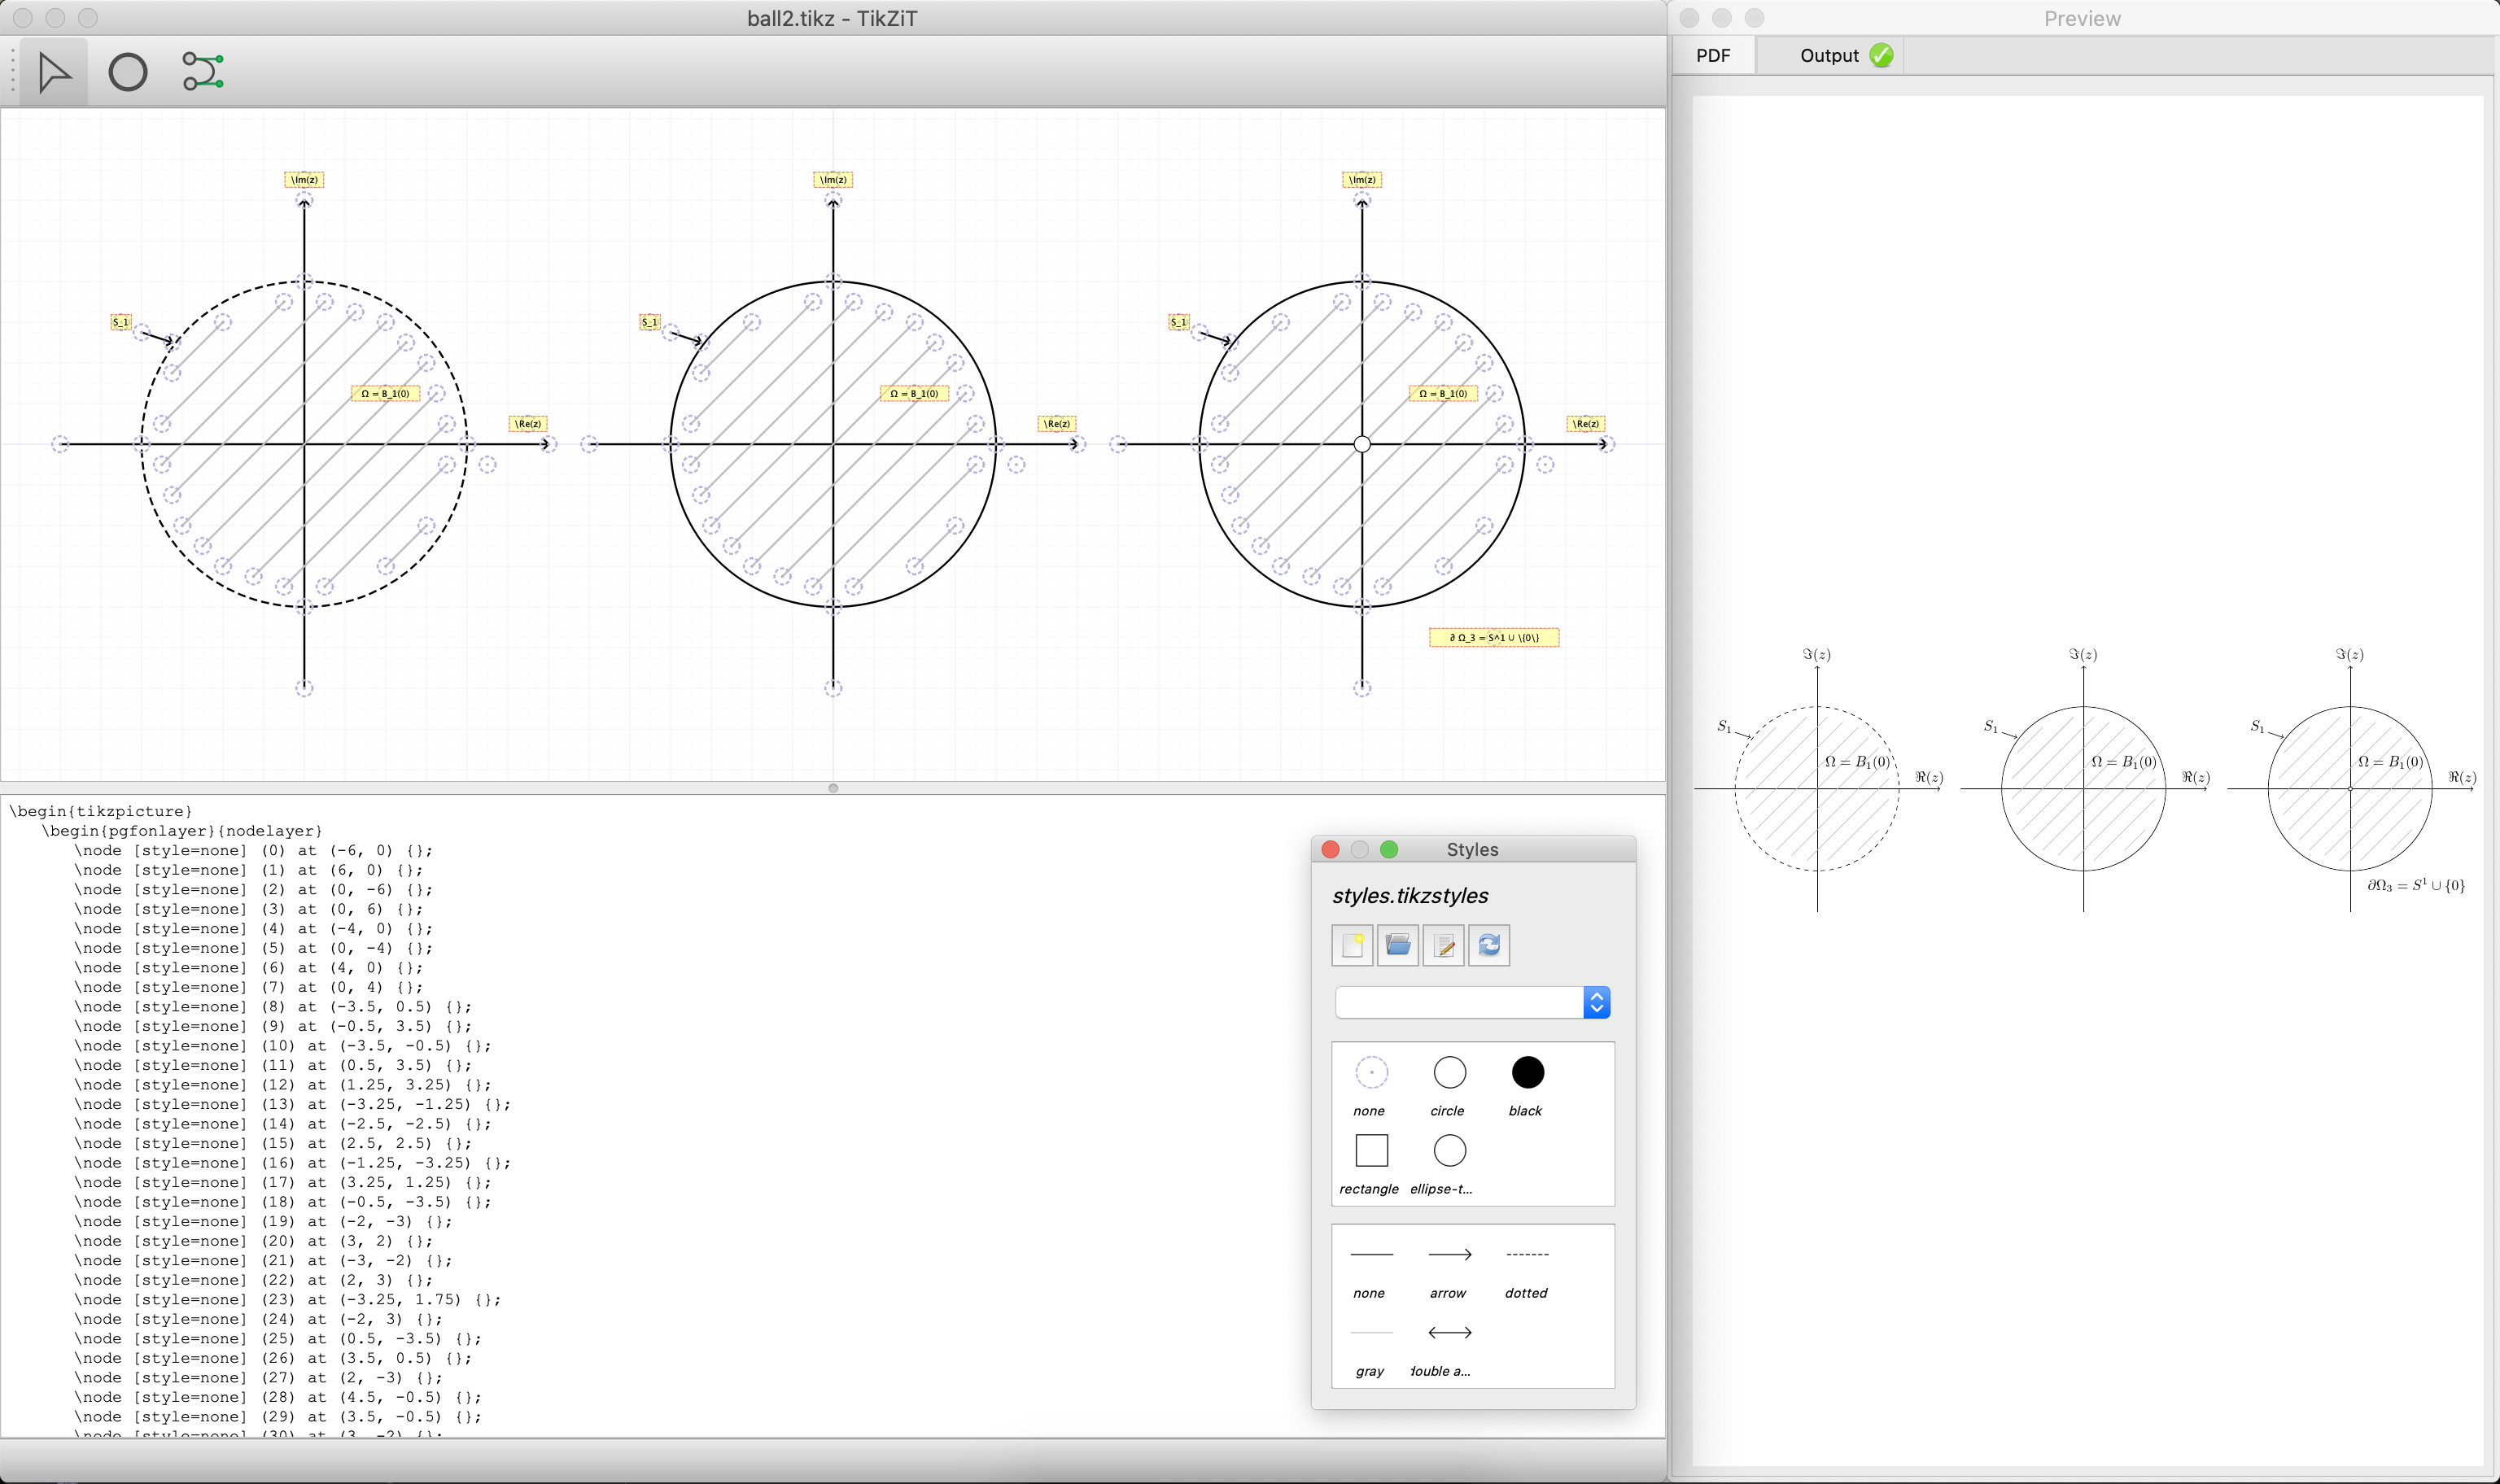
\includegraphics[width=0.8\textwidth]{figures/tikzit}	
	\end{figure}

\end{frame}

\section{Where to next?}

\begin{frame}{Congratulations!}
	\Large You can now write modular, clean documents without worrying (too much!) about page layout.
	
	You can write documents (papers, theses, even your assigments) easily and beautifully, and develop your own templates to suit your needs.
\end{frame}

\begin{frame}{Resources}
	\Large \LaTeX \ is a massive (and wonderful) rabbit hole. Jump in!
	
	\normalsize
	\begin{itemize}
	\item If you have any problems, visit the \textbf{TeX Stack Exchange} website (like Stack Overflow, but for TeX questions). \href{https://tex.stackexchange.com}{https://tex.stackexchange.com}	
	\item Read the LaTeX \textbf{Wikibook}! \href{https://en.wikibooks.org/wiki/LaTeX}{https://en.wikibooks.org/wiki/LaTeX}
	\item If you have any more questions, ask in the \textbf{UQCS Slack} channel \texttt{\#latex}, or you can DM me \texttt{@mcl}.
	\end{itemize}

\end{frame}

\section{Questions}

\begin{frame}
	\centering\Huge Questions?
\end{frame}

\end{document}
